%   +-------------+
%   |   RESULTS   |
%   +-------------+
\section{Results}\label{sec:result}

%   < Scheduling performance >
\subsection{Scheduling performance}\label{sec:res-sched}

\begin{figure}[p!]
    \centering
    \null\hfill
    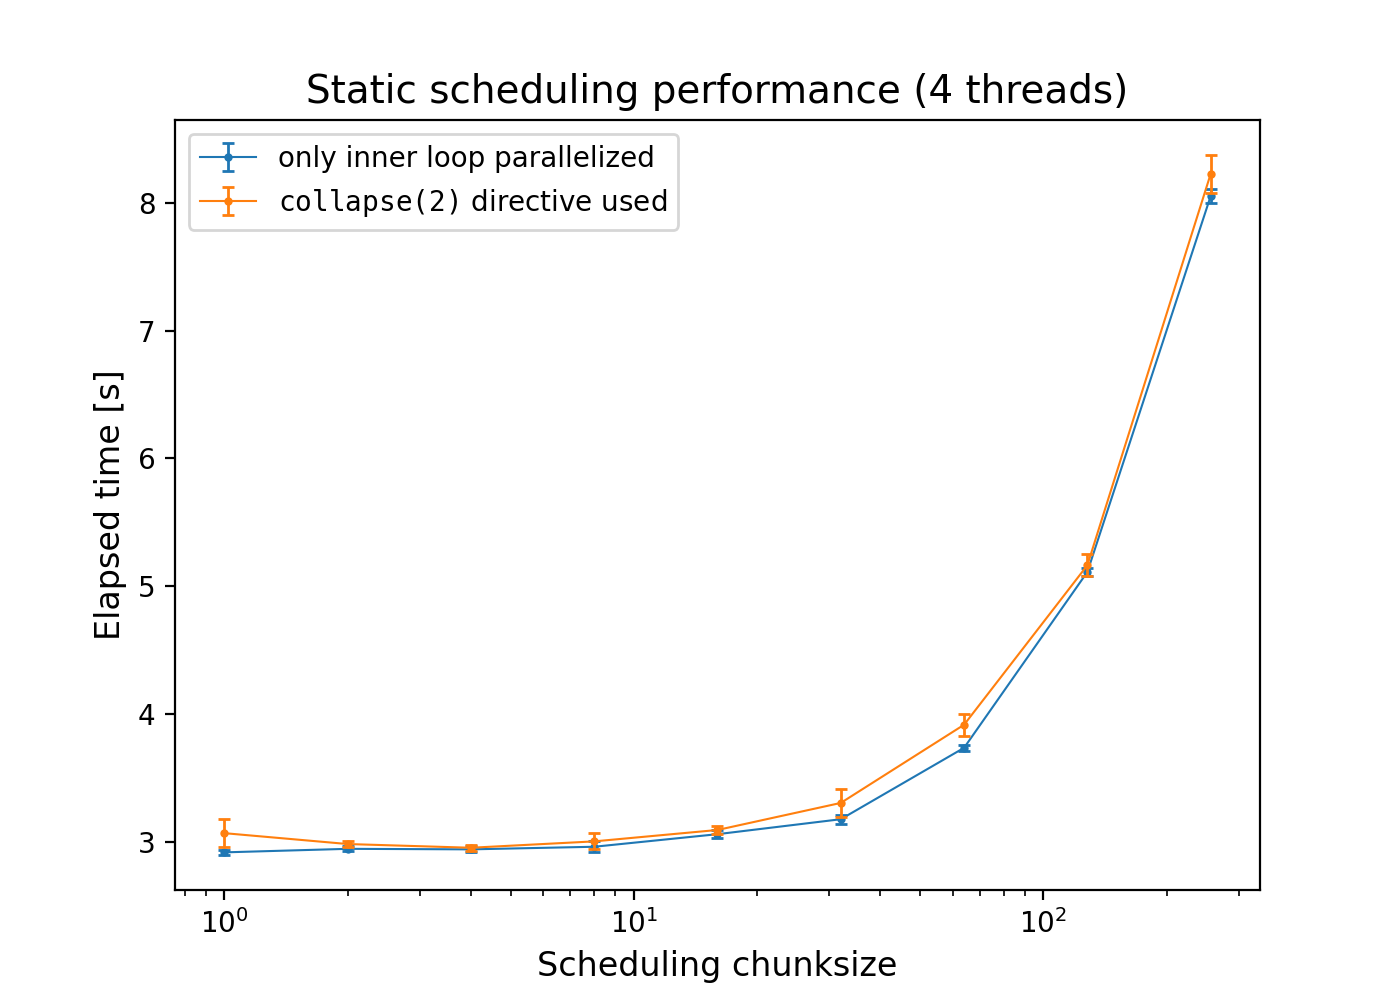
\includegraphics[width=0.49\textwidth]{sizeVStime_4threads_static.png}
    \null\hfill
    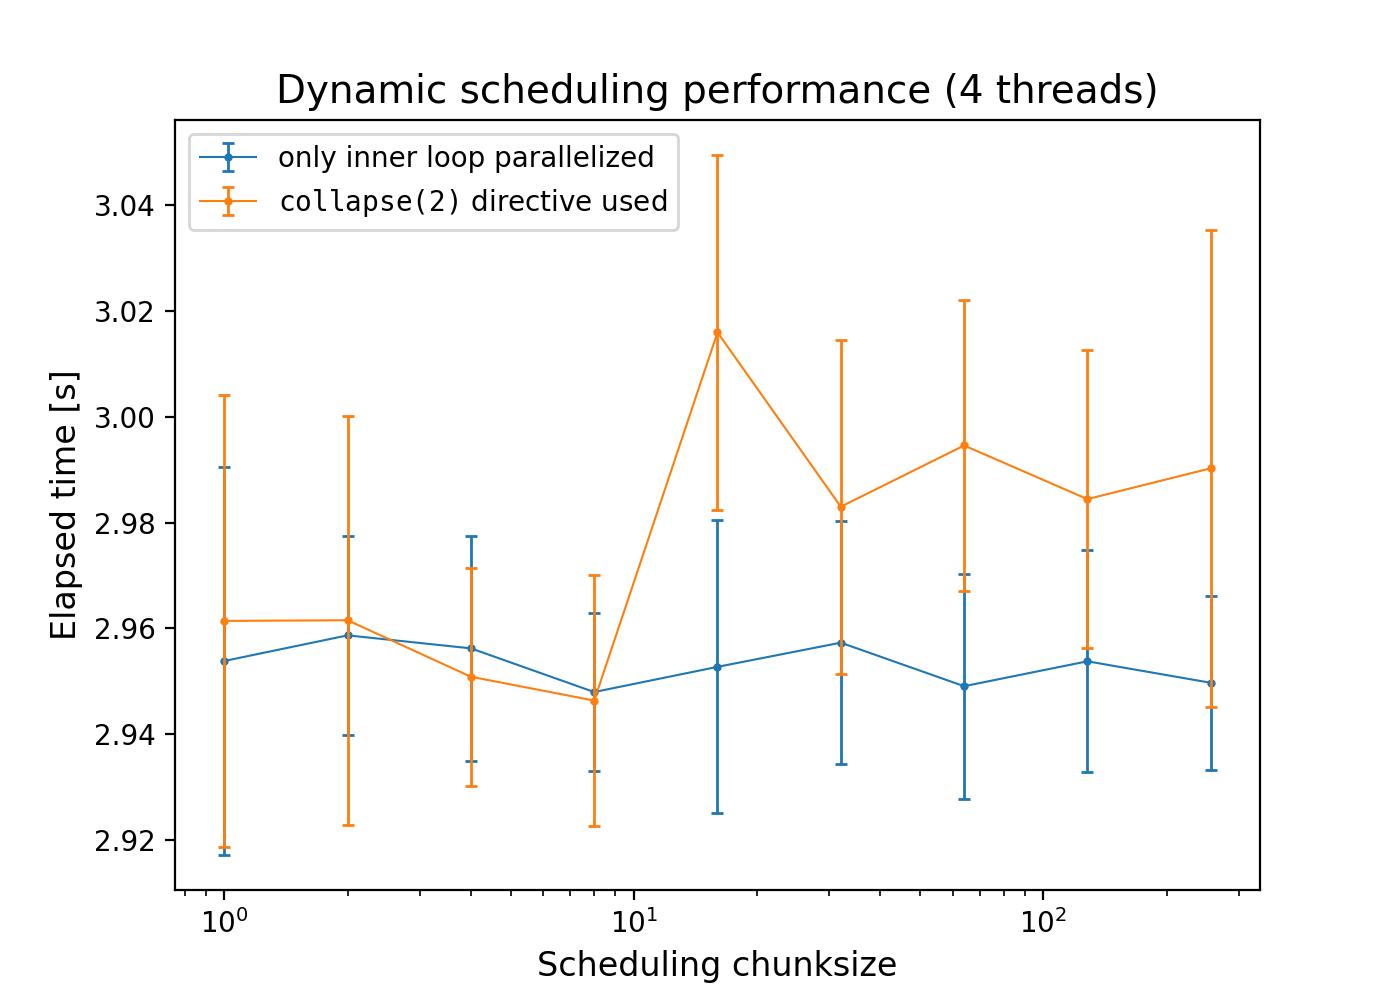
\includegraphics[width=0.49\textwidth]{sizeVStime_4threads_dynamic.png}
    \null\hfill
    \\
    \null\hfill
    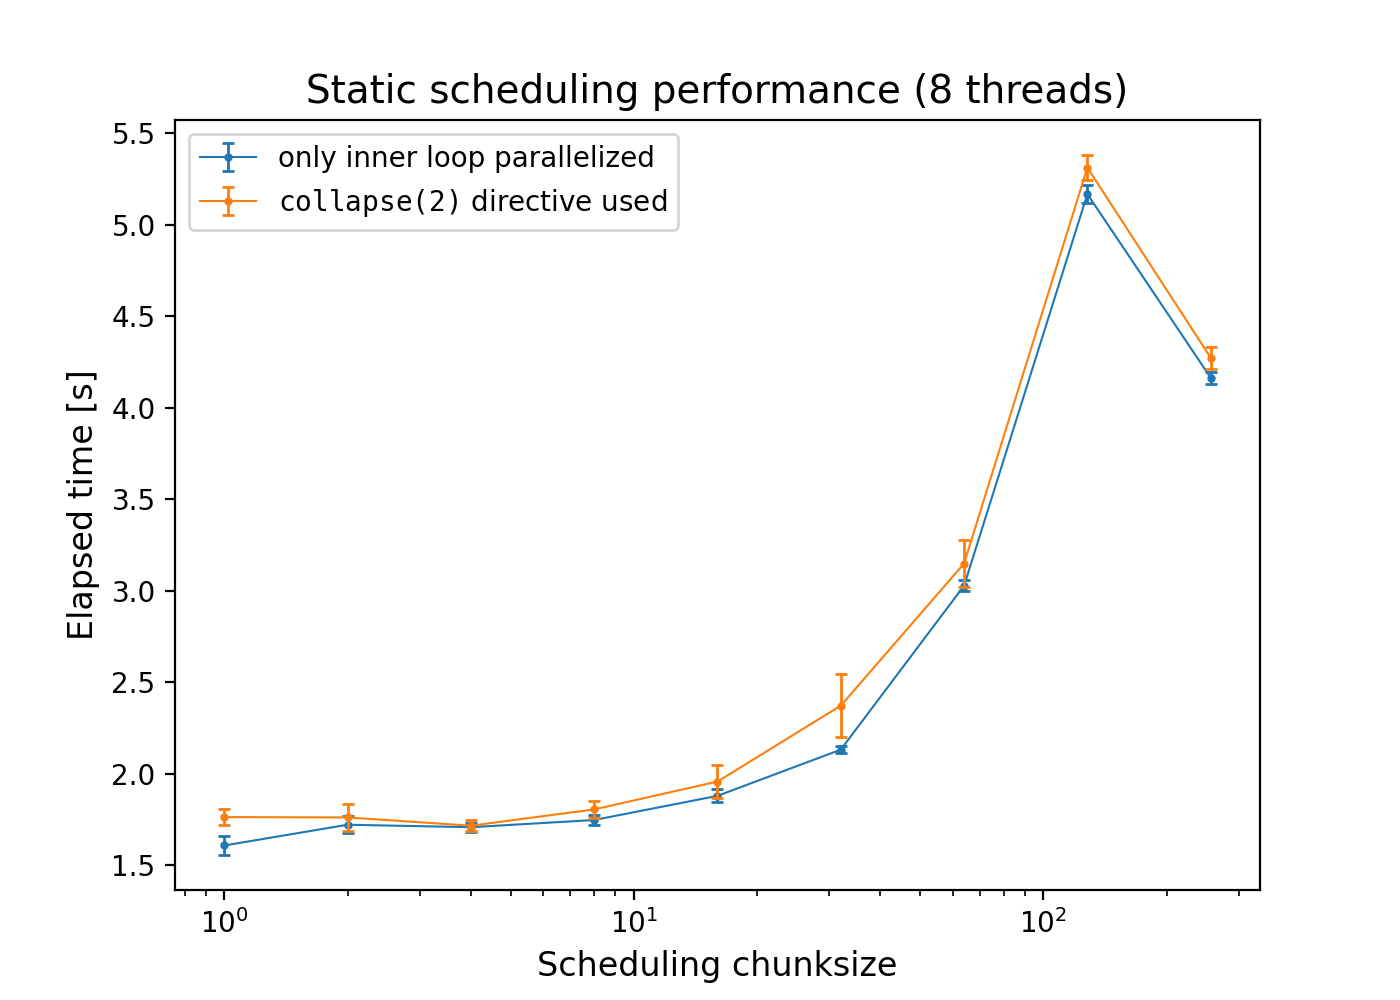
\includegraphics[width=0.49\textwidth]{sizeVStime_8threads_static.png}
    \null\hfill
    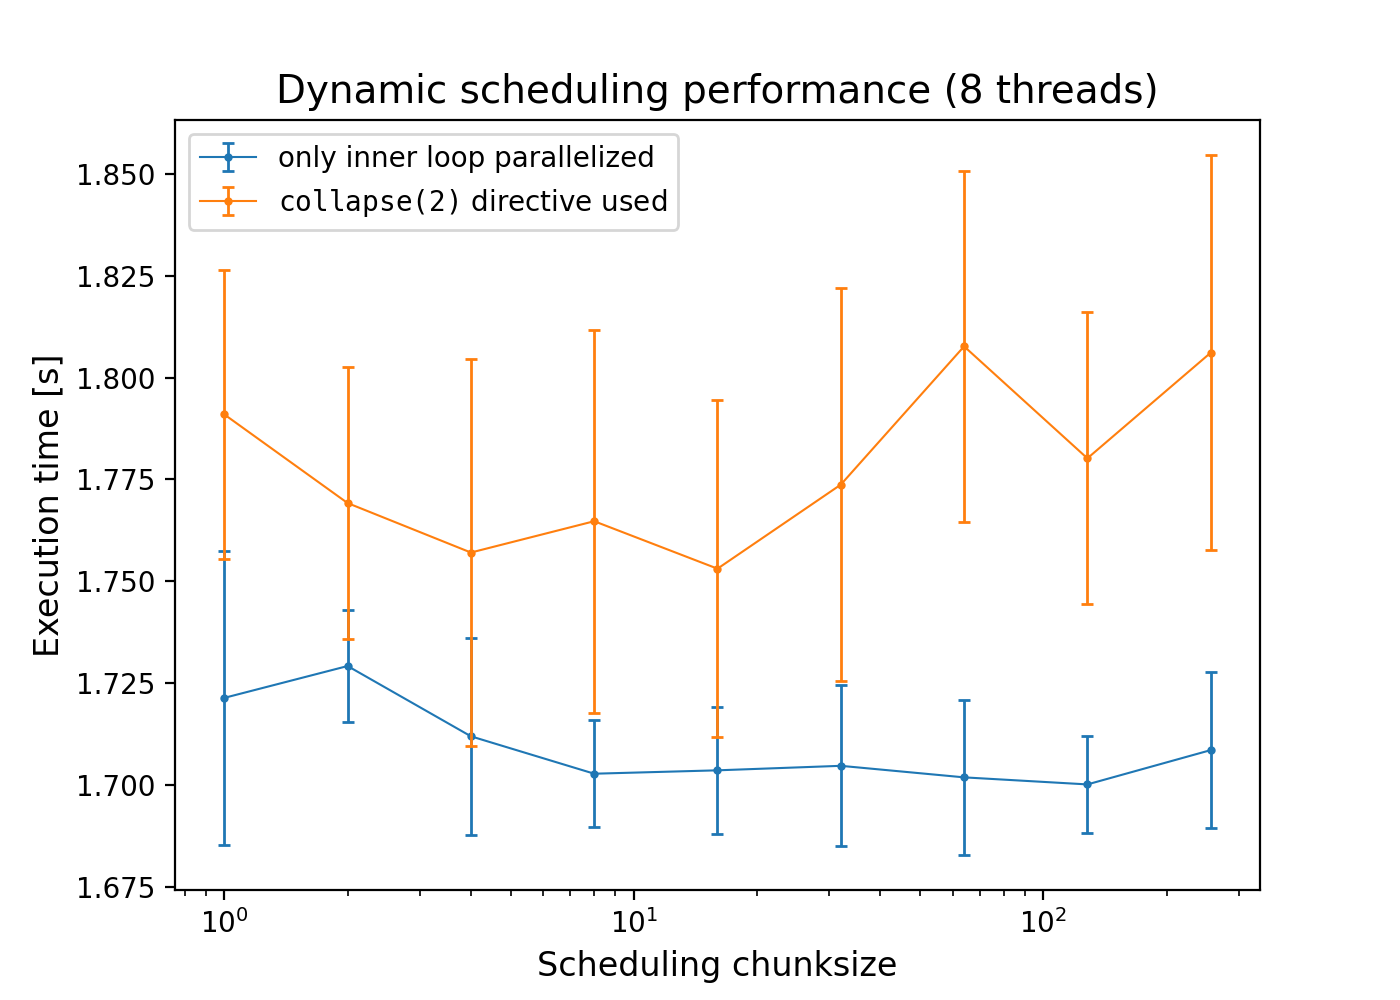
\includegraphics[width=0.49\textwidth]{sizeVStime_8threads_dynamic.png}
    \null\hfill
    \\
    \null\hfill
    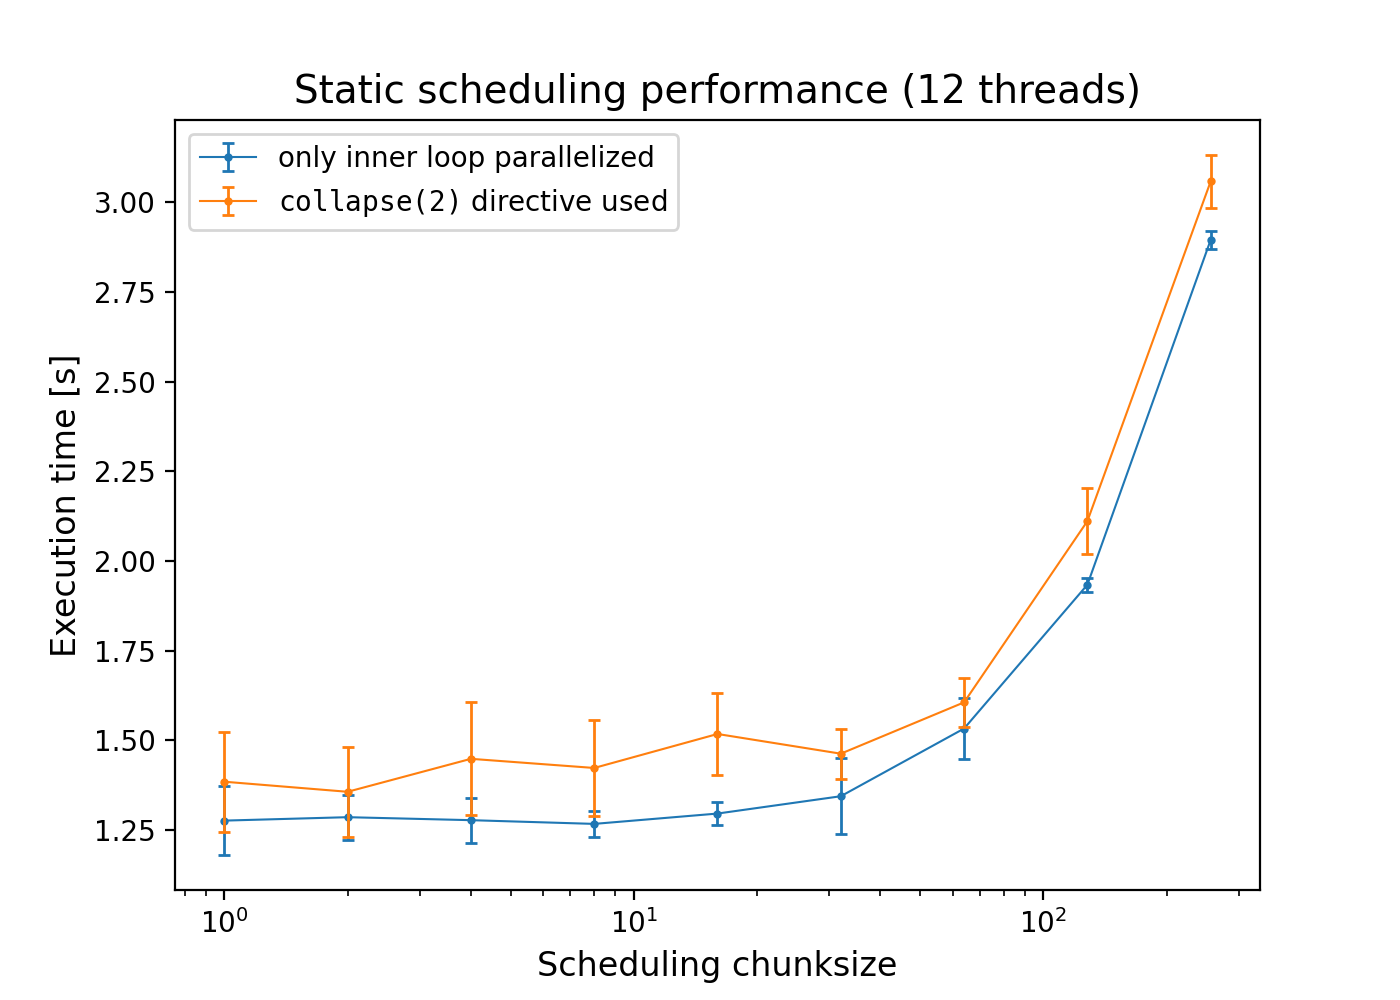
\includegraphics[width=0.49\textwidth]{sizeVStime_12threads_static.png}
    \null\hfill
    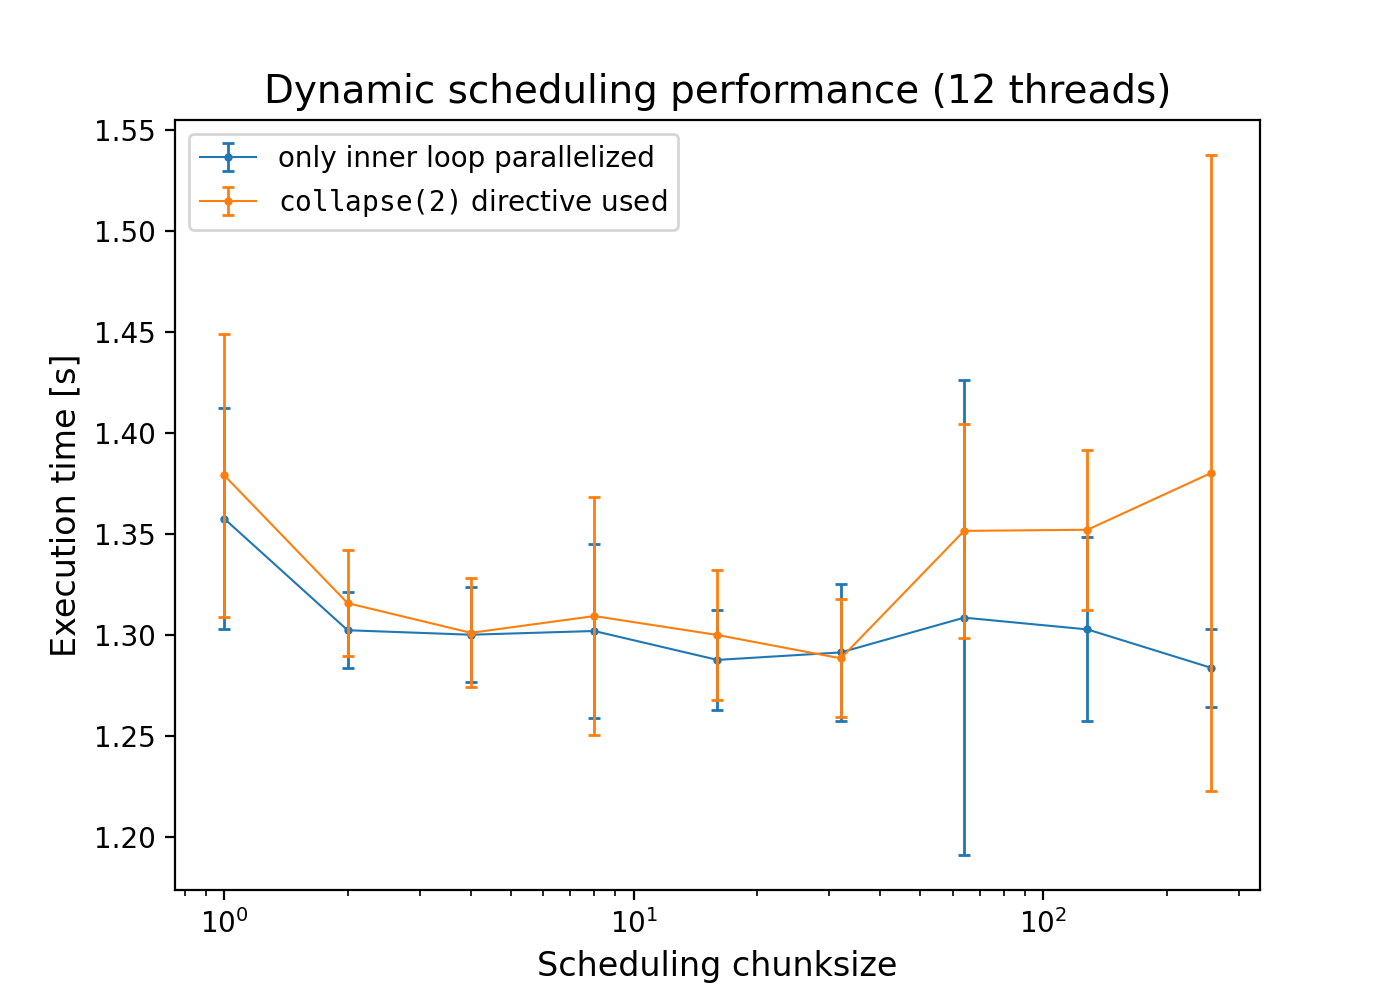
\includegraphics[width=0.49\textwidth]{sizeVStime_12threads_dynamic.png}
    \null\hfill
    \caption{\label{fig:sched}}
\end{figure}

The Figure~\ref{fig:sched} shows the time needed to compute the Mandelbrot set with respect to the partition size in \code{static} (left plots) and \code{dynamic} (right plots) scheduling conditions. Looking at the plots reported on the left column is clear that greater values of the scheduling chunksize leads to an increasing of the overhead. This is an expected behavior if we look at the graphical representation of the Mandelbrot set reported in Figure~\ref{fig:mandelbrot}: since the points with the highest computational cost are adjacent (the light brown ones), taking a large value for the chunksize corresponds to a high probability of assigning blocks of expensive computations to single threads, instead of distributing the workload as it happens with low values of the chunksize. On the contrary, the \code{dynamic} scheduling seems to be not affected by this drawback: a possible explanation is that the dynamic assignment of the workload allows to the quicker threads to handle the works more expensive, partially absorbing the overhead reported in \code{static} scheduling. However, I believe this isn't enough to describe what shown in the plots on the right column.

Another interesting results to derive from the plots in Figure~\ref{fig:sched} is a comparison in performance terms of the program with only the inner loop parallelized with respect to the the one that parallelizes the whole nested loop. Even in in most of the points the elapsed times seem to be consistent, the \code{collapse}-based program shows performance slightly worse than its counterpart. Again, we are looking at a non-completely understood behavior that maybe can be described like a sort of edge-phenomenon: in fact, the \ompcode{collapse(2)} clause allows to unroll the nested loop, leading the last iterations of the outer loop to be adjacent to the first ones of the next inner loop. Since the region near the edges almost doesn't require any computation (see the colors of the Figure~\ref{fig:mandelbrot}), it can lead to a greater probability of having the \emph{same} processors to perform the heaviest work, for both \code{static} and \code{dynamic} scheduling. 

%   < Weak and strong scaling performance >
\subsection{Weak and strong scaling performance}\label{sec:res-scale}

\begin{figure}[h!]
    \centering
    \null\hfill
    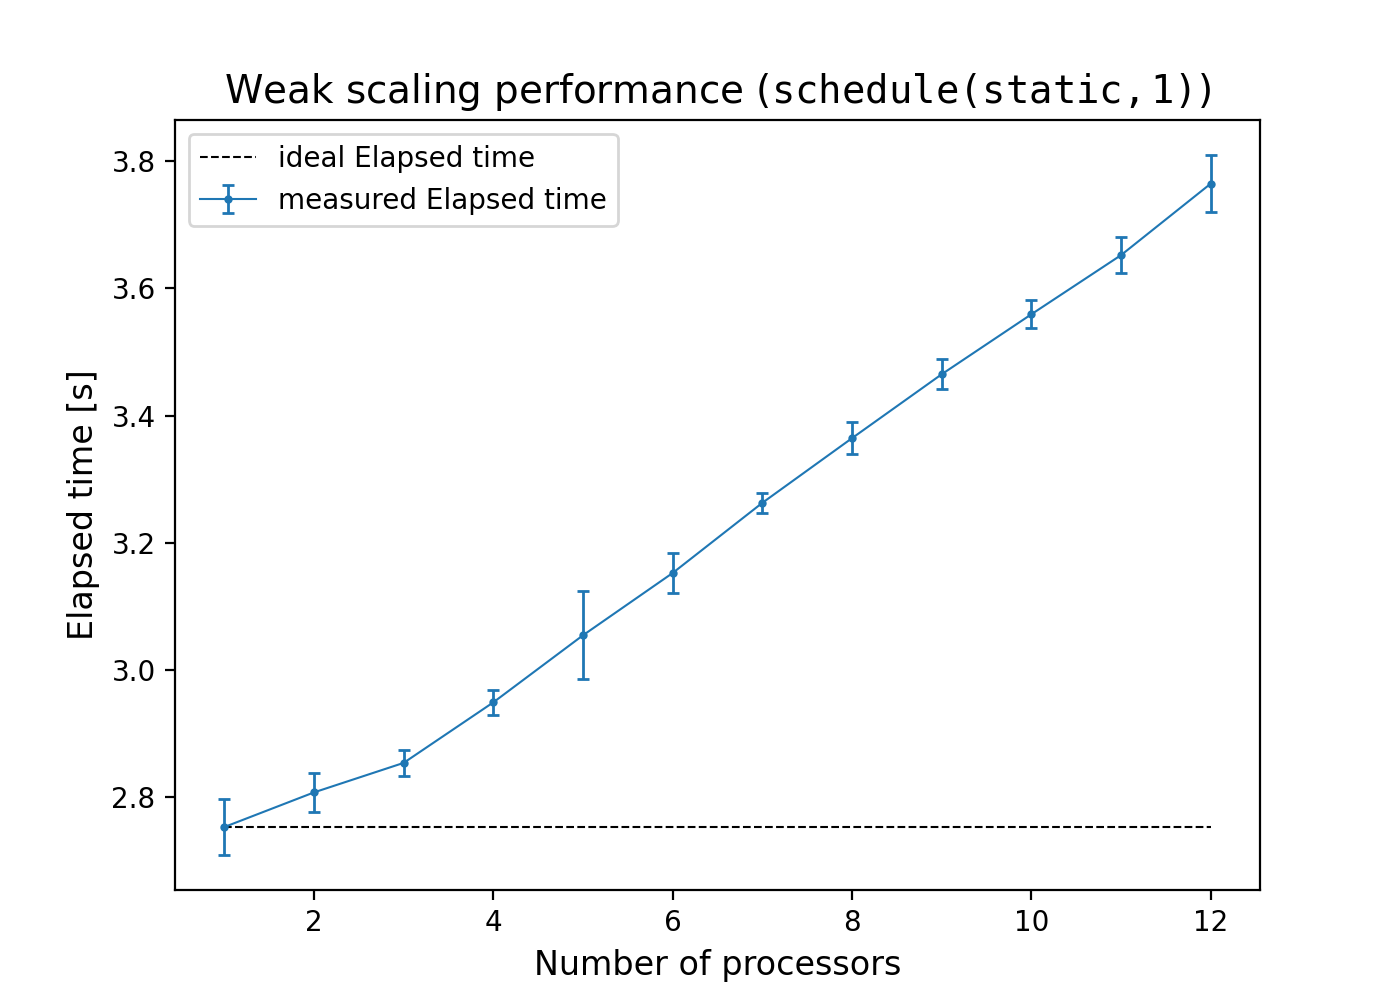
\includegraphics[width=0.45\textwidth]{threadsVStime_weak.png}
    \null\hfill
    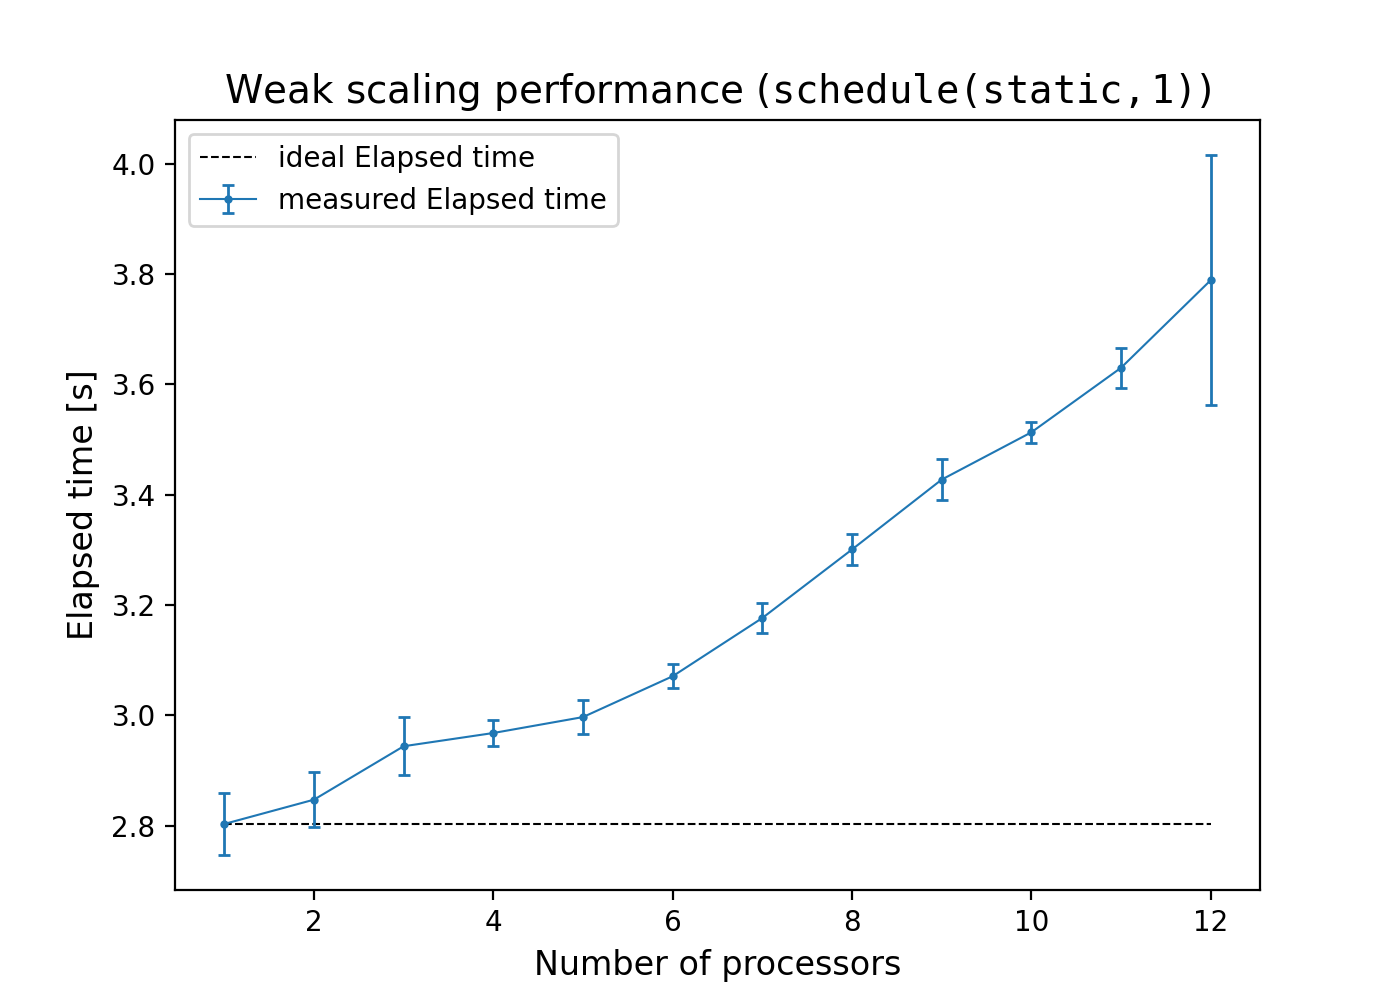
\includegraphics[width=0.45\textwidth]{threadsVStime_weak_collapse.png}
    \null\hfill
    \\
    \null\hfill
    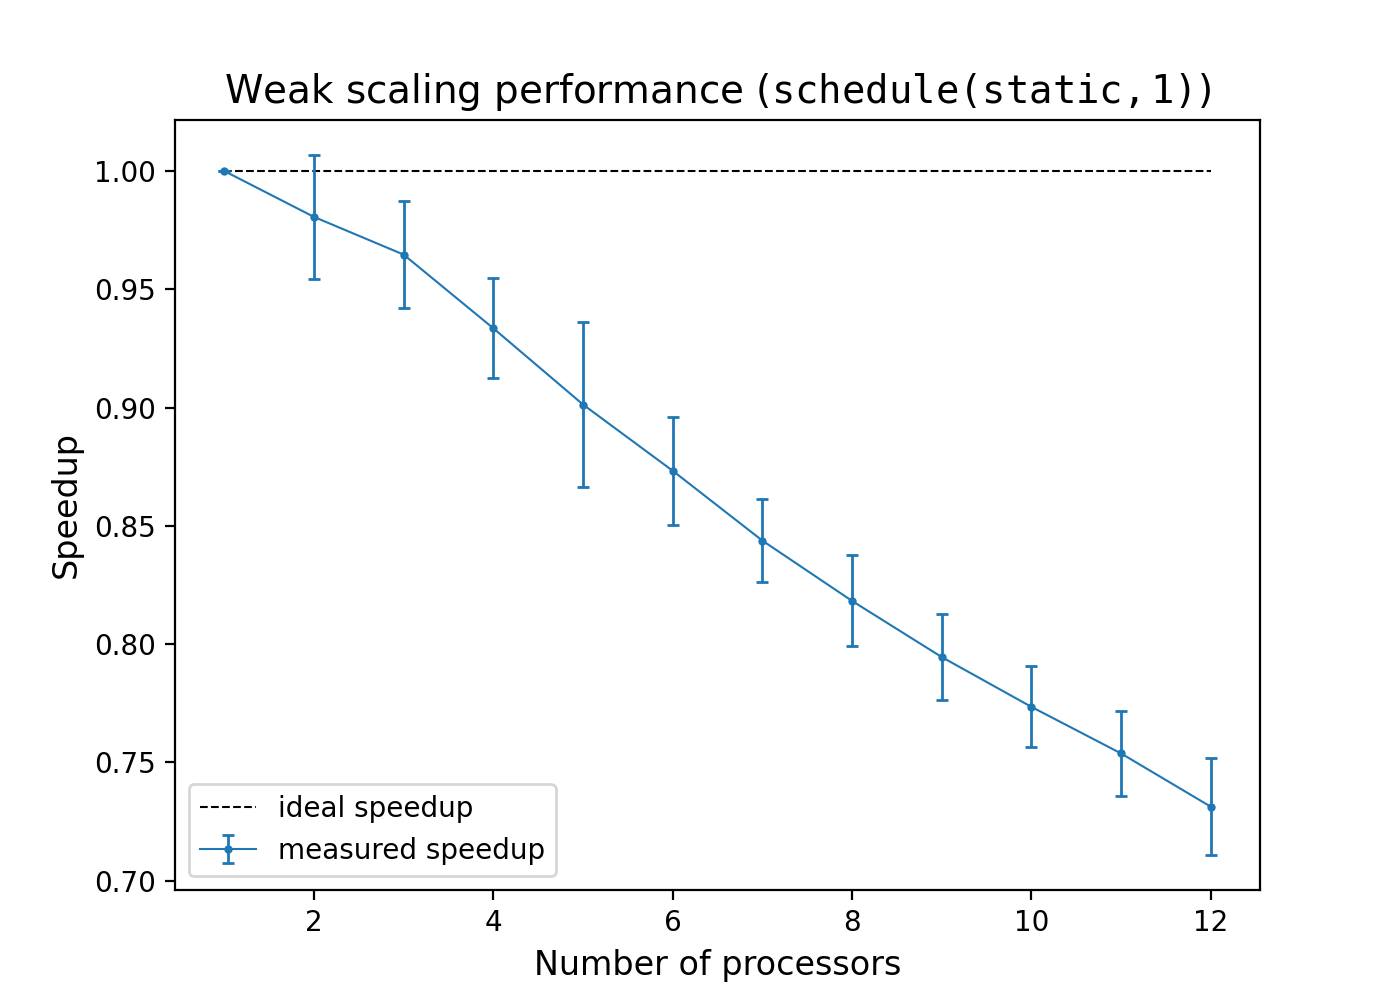
\includegraphics[width=0.45\textwidth]{threadsVSspeedup_weak.png}
    \null\hfill
    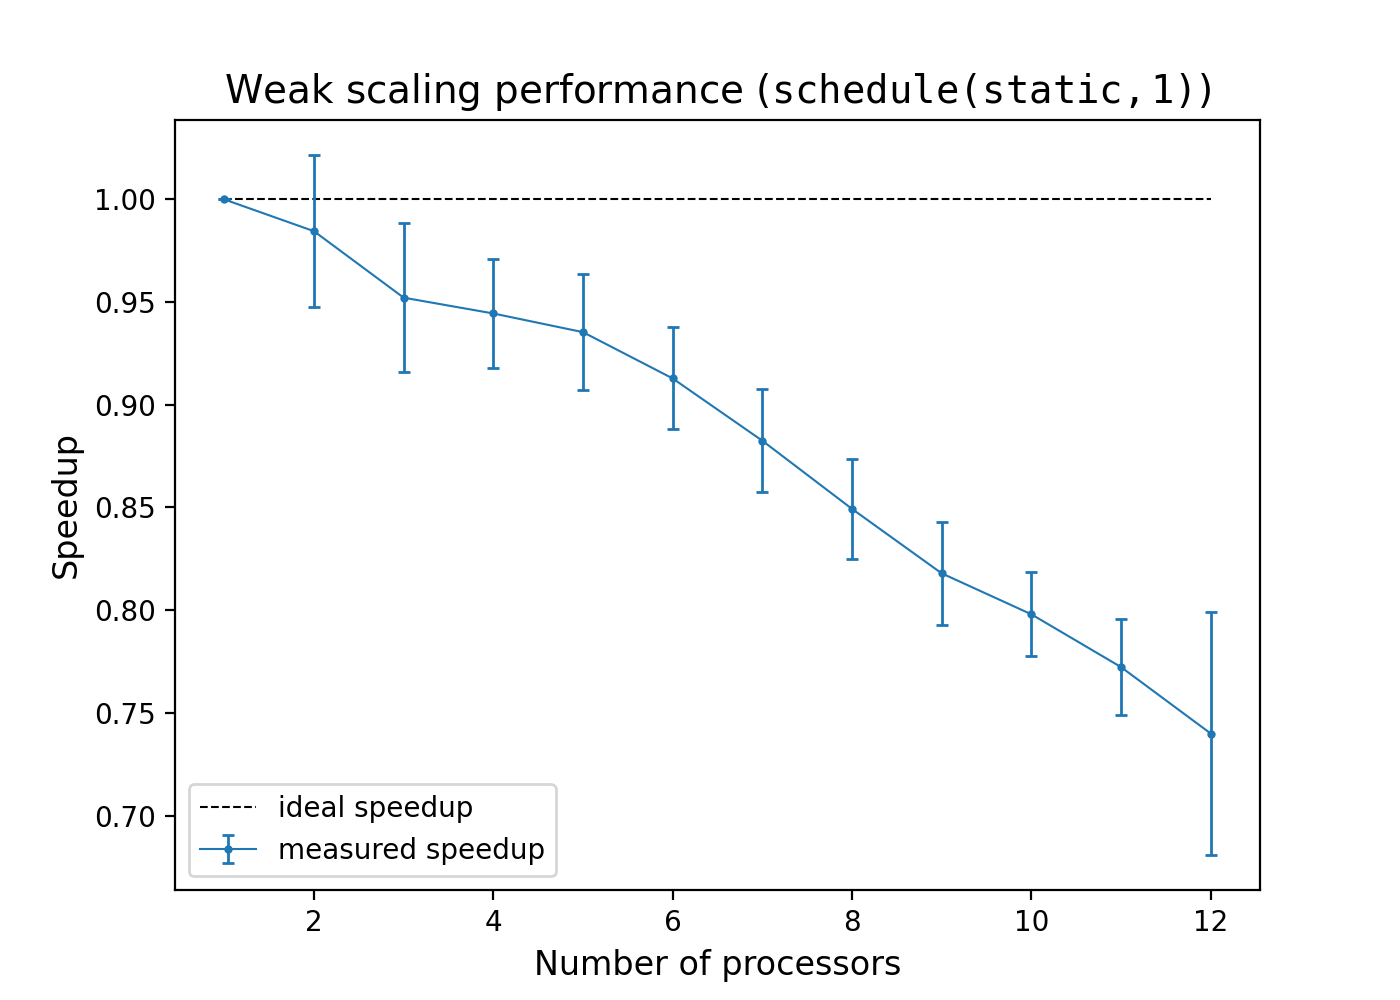
\includegraphics[width=0.45\textwidth]{threadsVSspeedup_weak_collapse.png}
    \null\hfill
    \caption{\label{fig:strong_scale}}
\end{figure}

\begin{figure}[h!]
    \centering
    \null\hfill
    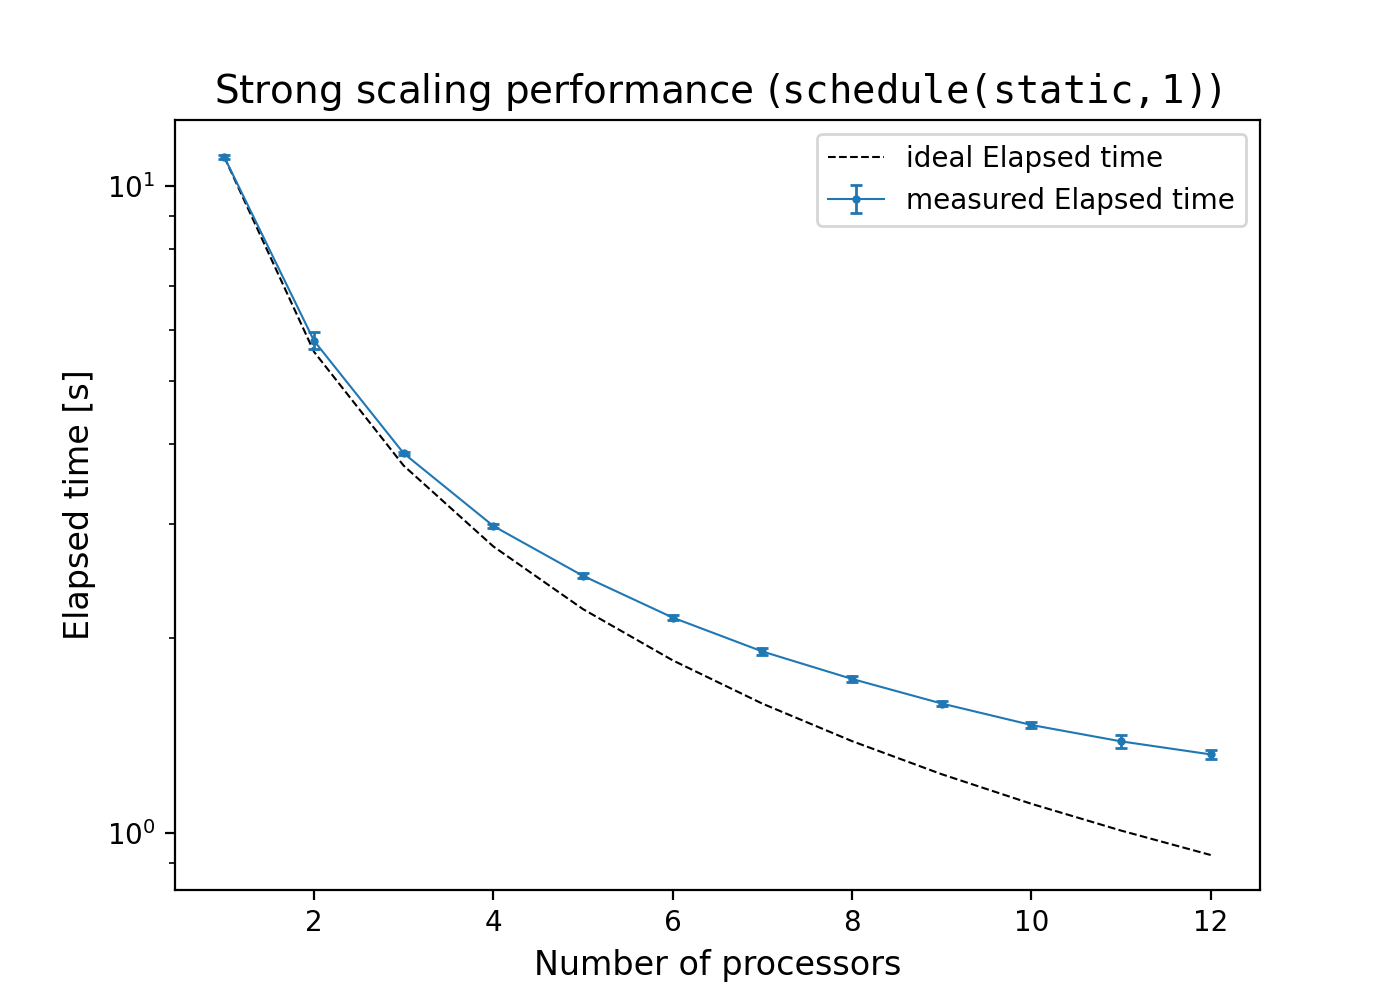
\includegraphics[width=0.45\textwidth]{threadsVStime_strong.png}
    \null\hfill
    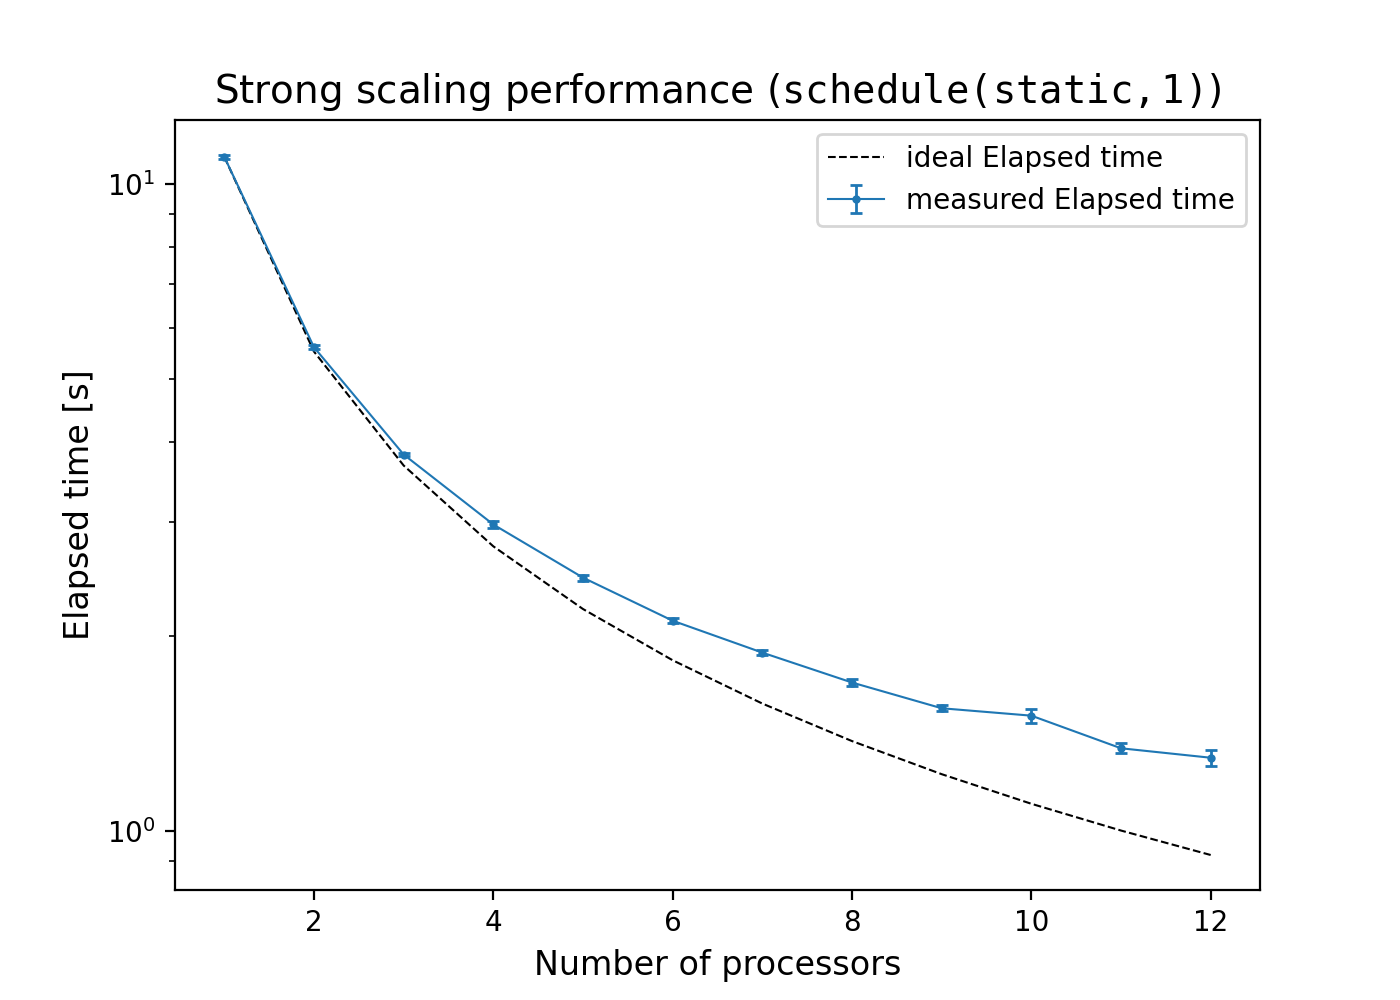
\includegraphics[width=0.45\textwidth]{threadsVStime_strong_collapse.png}
    \null\hfill
    \\
    \null\hfill
    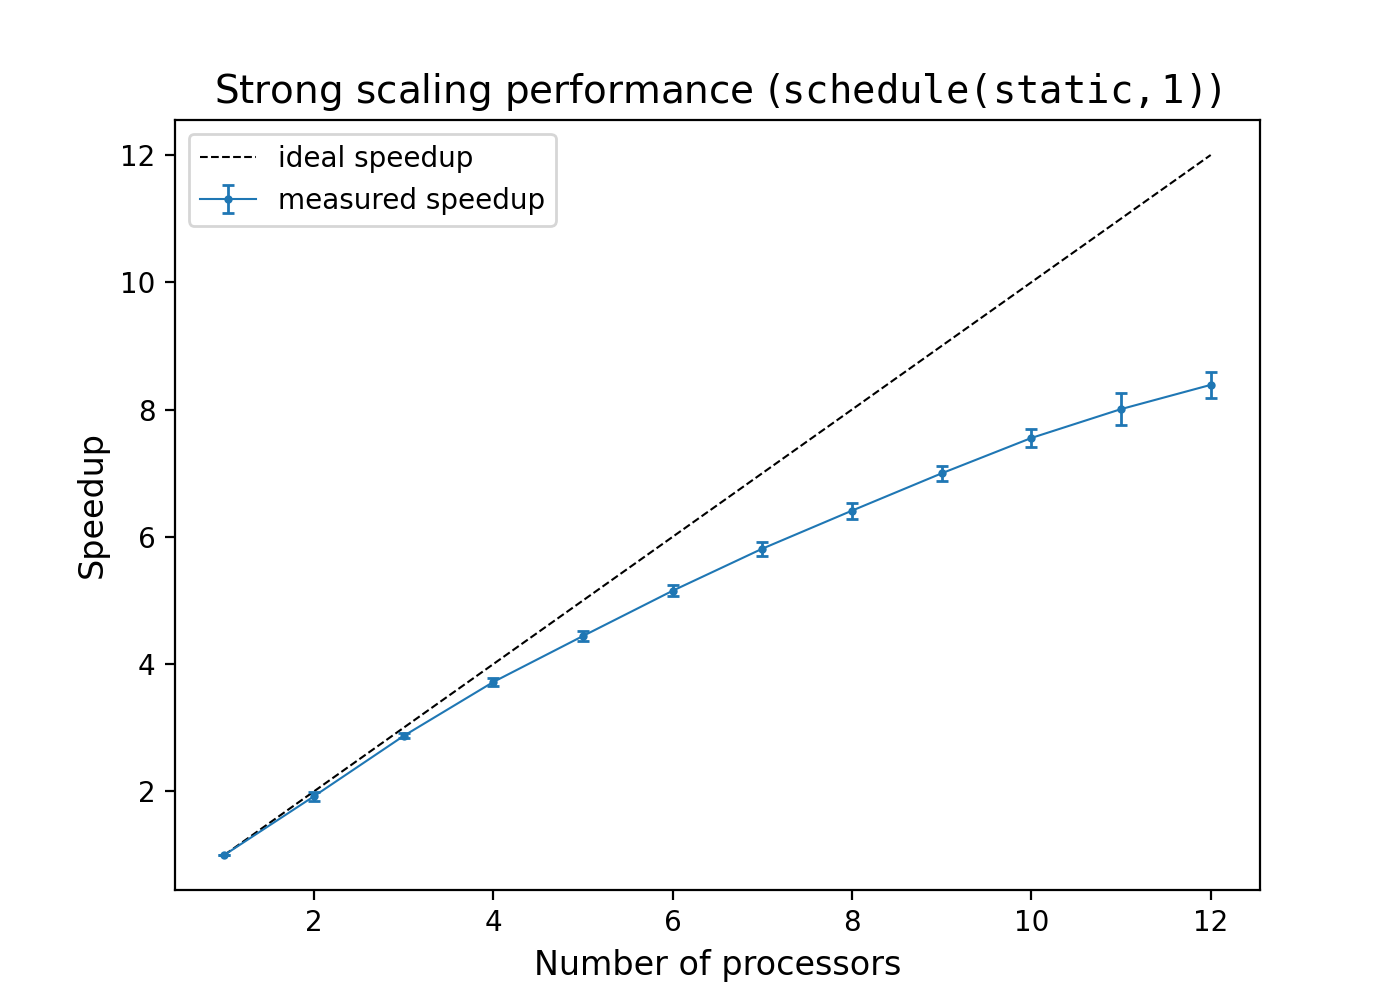
\includegraphics[width=0.45\textwidth]{threadsVSspeedup_strong.png}
    \null\hfill
    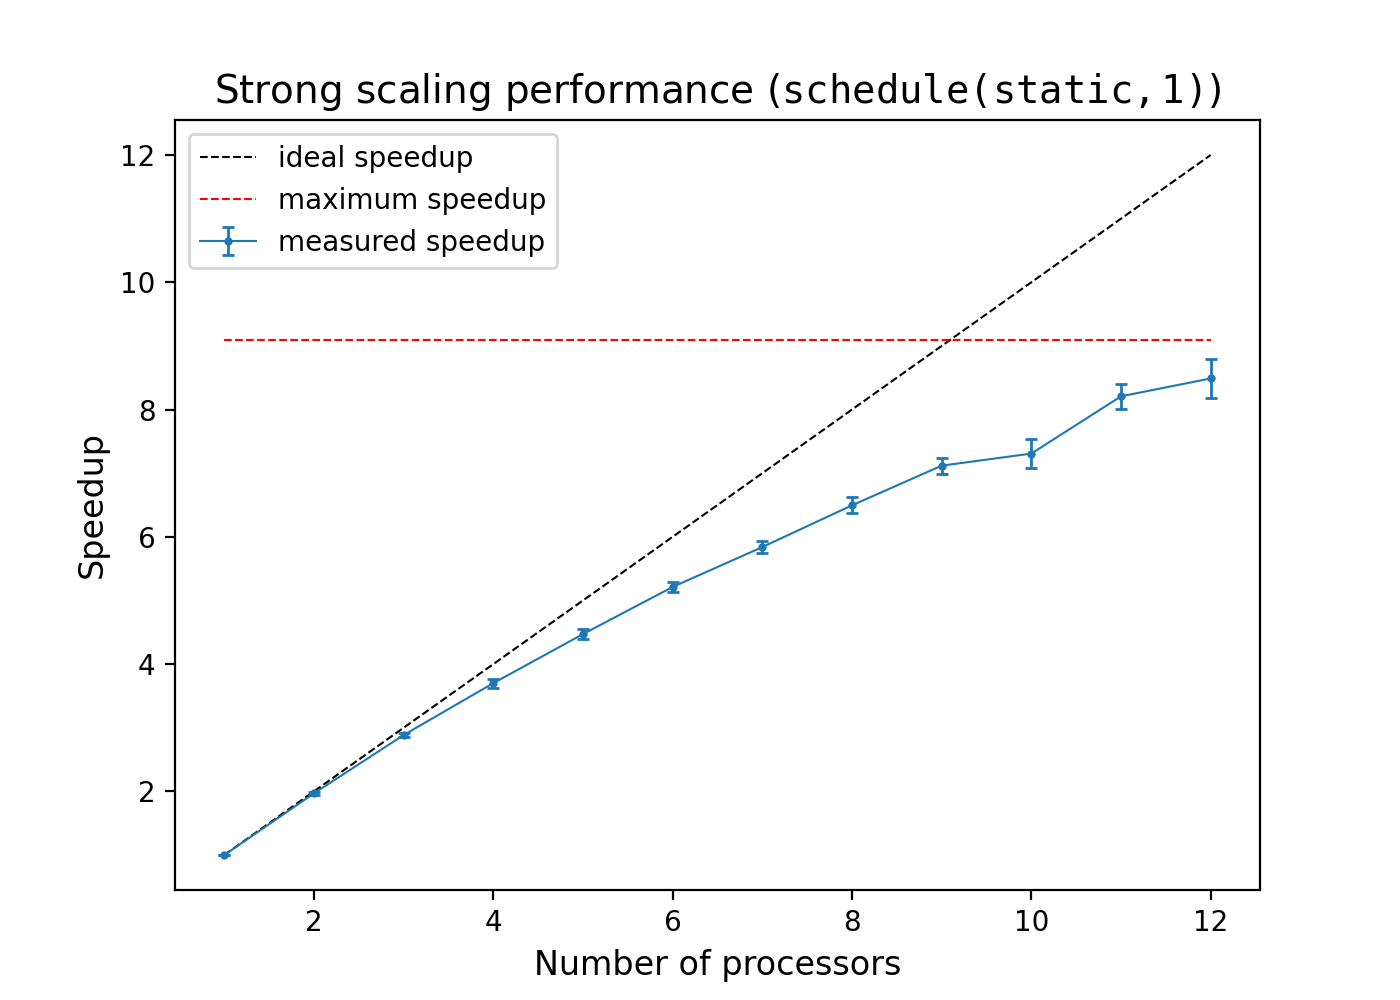
\includegraphics[width=0.45\textwidth]{threadsVSspeedup_strong_collapse.png}
    \null\hfill
    \caption{\label{fig:strong_scale}}
\end{figure}
